\documentclass{article}
\usepackage{fontspec,tikz,graphicx}
\setmainfont{Times New Roman}
\usepackage[a3paper,margin=1cm]{geometry}
\pagestyle{empty}
\begin{document}
\noindent\resizebox{\textwidth}{!}{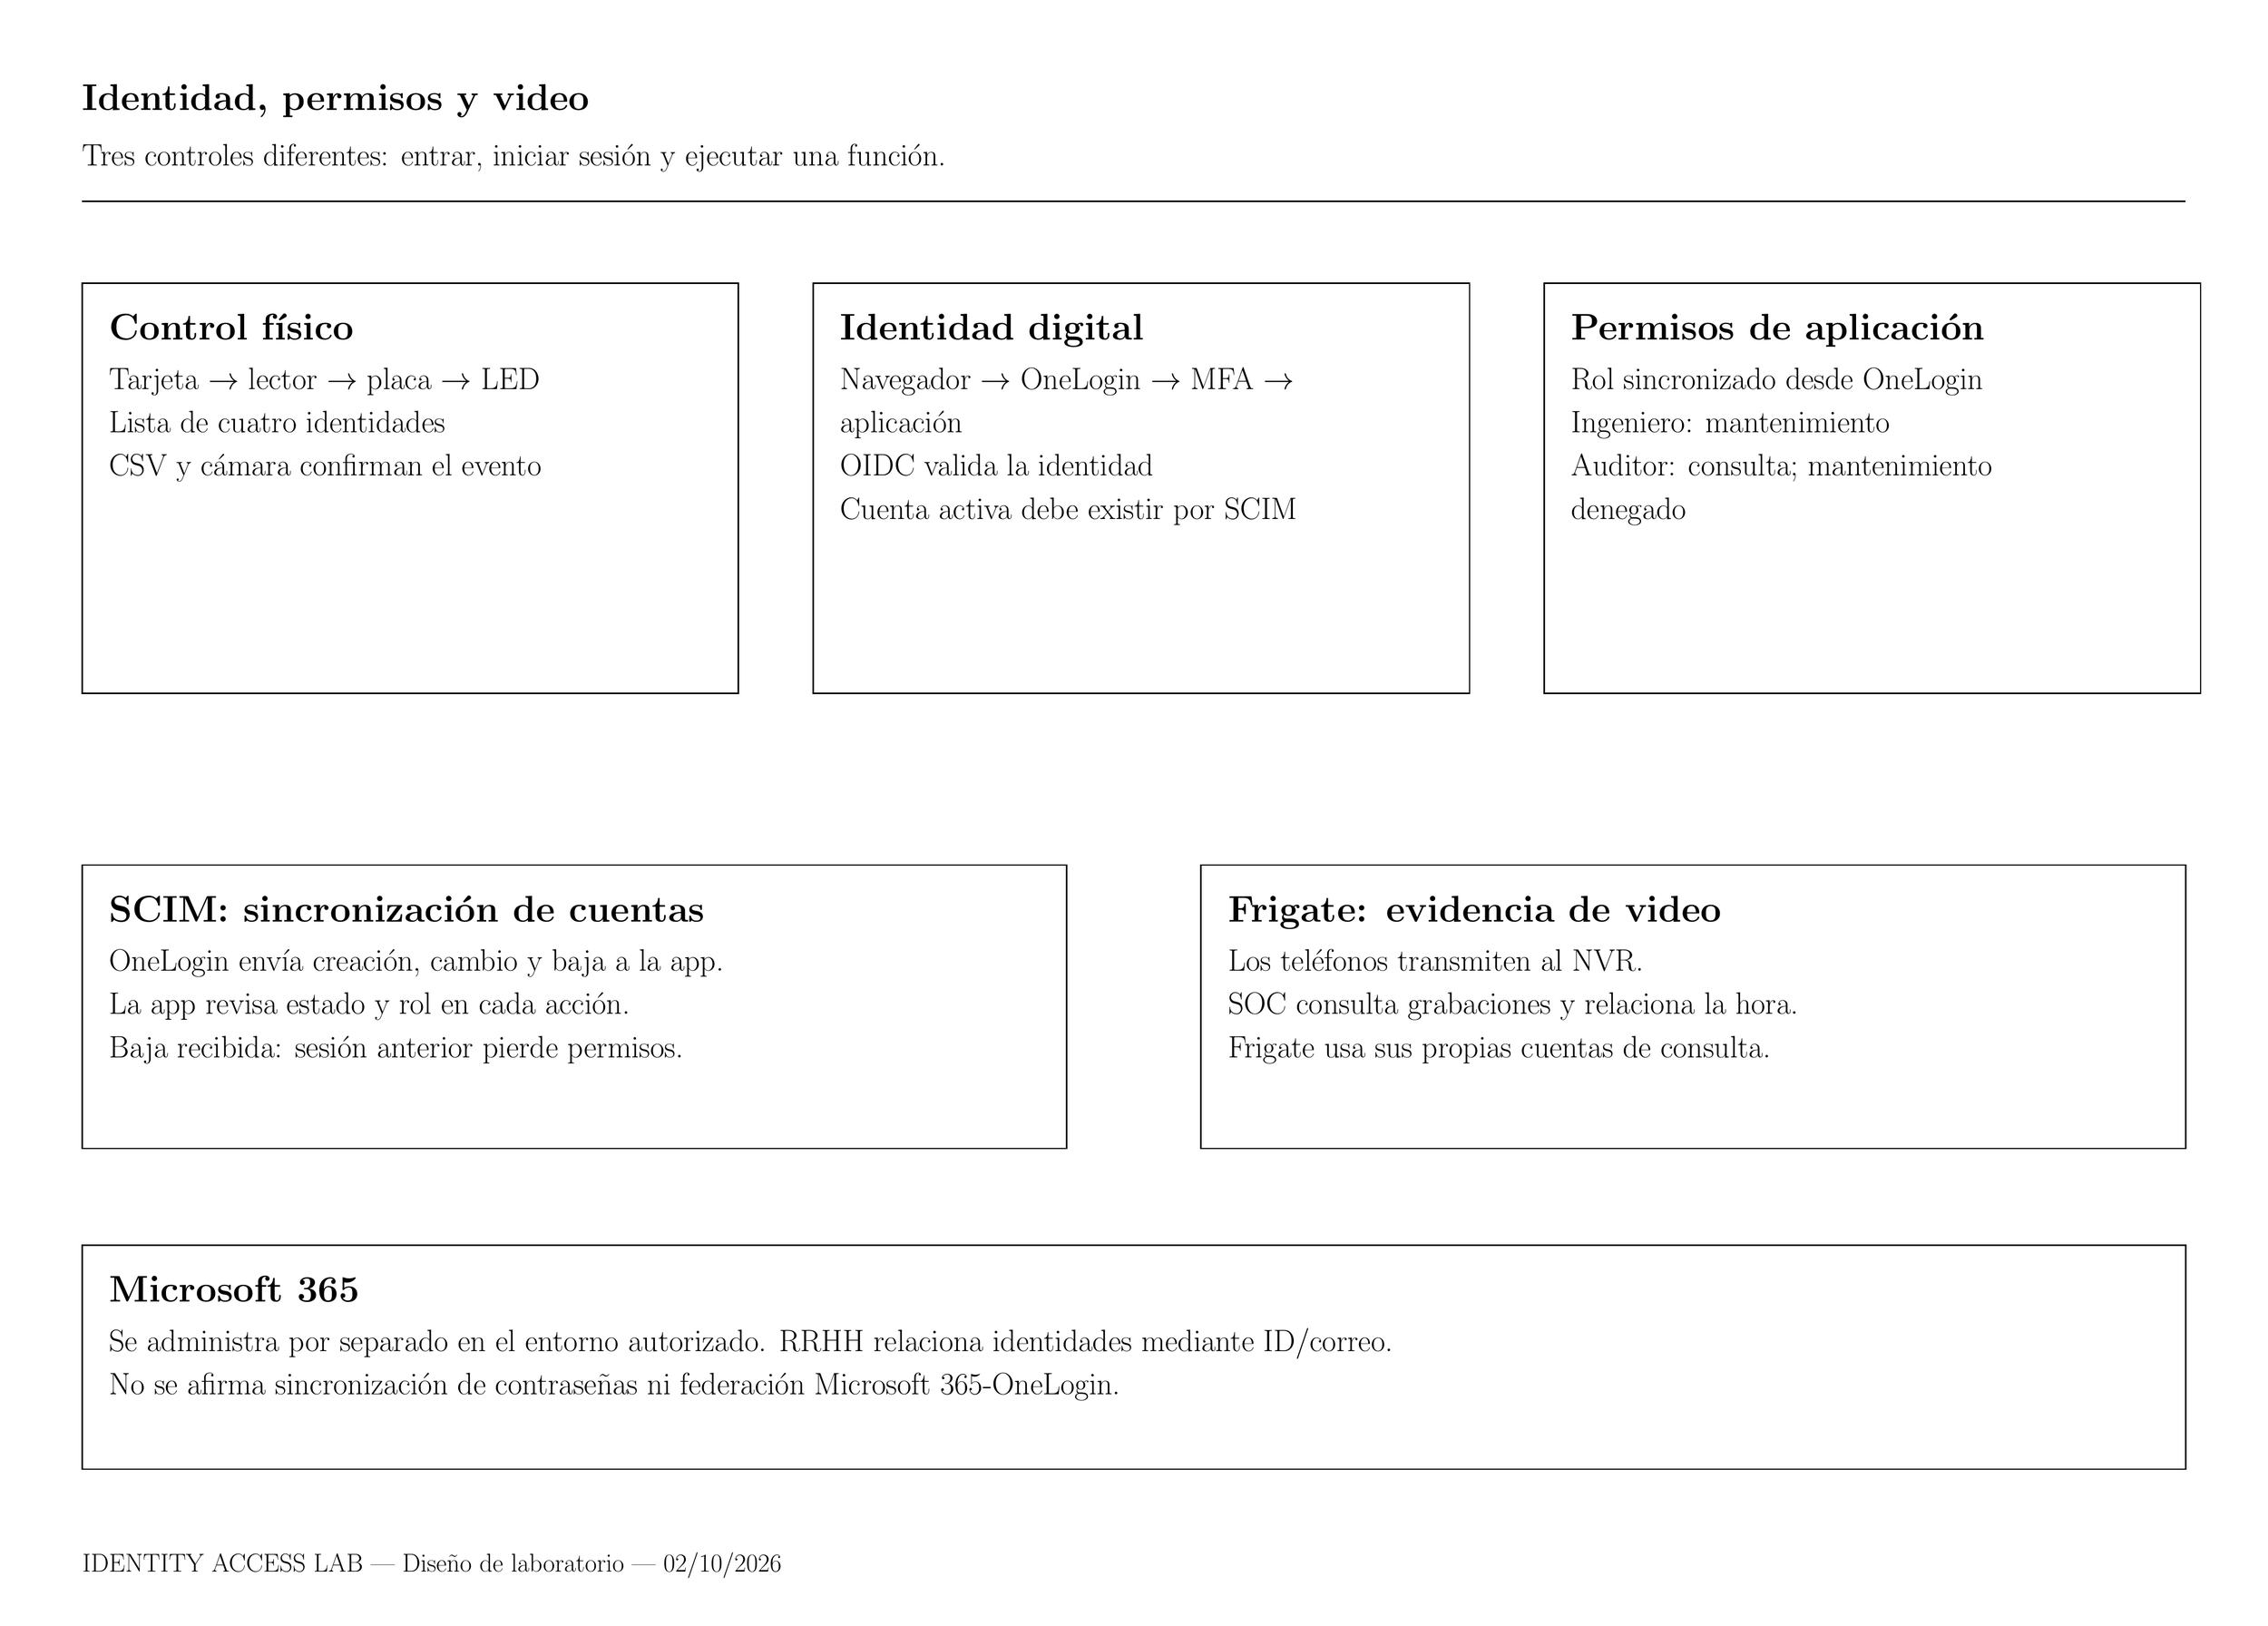
\begin{tikzpicture}[x=1pt,y=-1pt]
\path[use as bounding box] (0,0) rectangle (1500.0,1070.0);
\node[anchor=base west,inner sep=0pt,font=\fontsize{34.0}{40.8}\selectfont \bfseries ] at (45,64) {Identidad, permisos y video};
\node[anchor=base west,inner sep=0pt,font=\fontsize{21.0}{25.2}\selectfont ] at (45,101) {Tres controles diferentes: entrar, iniciar sesión y ejecutar una función.};
\draw[line width=1pt] (45,125) -- (1455,125);
\draw[line width=1pt] (45.0,180.0) rectangle (485.0,455.0);
\node[anchor=base west,inner sep=0pt,font=\fontsize{24.0}{28.799999999999997}\selectfont \bfseries ] at (63,218) {Control físico};
\node[anchor=base west,inner sep=0pt,font=\fontsize{22.0}{26.4}\selectfont ] at (63,251) {Tarjeta \(\rightarrow\) lector \(\rightarrow\) placa \(\rightarrow\) LED};
\node[anchor=base west,inner sep=0pt,font=\fontsize{22.0}{26.4}\selectfont ] at (63,280) {Lista de cuatro identidades};
\node[anchor=base west,inner sep=0pt,font=\fontsize{22.0}{26.4}\selectfont ] at (63,309) {CSV y cámara confirman el evento};
\draw[line width=1pt] (535.0,180.0) rectangle (975.0,455.0);
\node[anchor=base west,inner sep=0pt,font=\fontsize{24.0}{28.799999999999997}\selectfont \bfseries ] at (553,218) {Identidad digital};
\node[anchor=base west,inner sep=0pt,font=\fontsize{22.0}{26.4}\selectfont ] at (553,251) {Navegador \(\rightarrow\) OneLogin \(\rightarrow\) MFA \(\rightarrow\)};
\node[anchor=base west,inner sep=0pt,font=\fontsize{22.0}{26.4}\selectfont ] at (553,280) {aplicación};
\node[anchor=base west,inner sep=0pt,font=\fontsize{22.0}{26.4}\selectfont ] at (553,309) {OIDC valida la identidad};
\node[anchor=base west,inner sep=0pt,font=\fontsize{22.0}{26.4}\selectfont ] at (553,338) {Cuenta activa debe existir por SCIM};
\draw[line width=1pt] (1025.0,180.0) rectangle (1465.0,455.0);
\node[anchor=base west,inner sep=0pt,font=\fontsize{24.0}{28.799999999999997}\selectfont \bfseries ] at (1043,218) {Permisos de aplicación};
\node[anchor=base west,inner sep=0pt,font=\fontsize{22.0}{26.4}\selectfont ] at (1043,251) {Rol sincronizado desde OneLogin};
\node[anchor=base west,inner sep=0pt,font=\fontsize{22.0}{26.4}\selectfont ] at (1043,280) {Ingeniero: mantenimiento};
\node[anchor=base west,inner sep=0pt,font=\fontsize{22.0}{26.4}\selectfont ] at (1043,309) {Auditor: consulta; mantenimiento};
\node[anchor=base west,inner sep=0pt,font=\fontsize{22.0}{26.4}\selectfont ] at (1043,338) {denegado};
\draw[line width=1pt] (45.0,570.0) rectangle (705.0,760.0);
\node[anchor=base west,inner sep=0pt,font=\fontsize{24.0}{28.799999999999997}\selectfont \bfseries ] at (63,608) {SCIM: sincronización de cuentas};
\node[anchor=base west,inner sep=0pt,font=\fontsize{22.0}{26.4}\selectfont ] at (63,641) {OneLogin envía creación, cambio y baja a la app.};
\node[anchor=base west,inner sep=0pt,font=\fontsize{22.0}{26.4}\selectfont ] at (63,670) {La app revisa estado y rol en cada acción.};
\node[anchor=base west,inner sep=0pt,font=\fontsize{22.0}{26.4}\selectfont ] at (63,699) {Baja recibida: sesión anterior pierde permisos.};
\draw[line width=1pt] (795.0,570.0) rectangle (1455.0,760.0);
\node[anchor=base west,inner sep=0pt,font=\fontsize{24.0}{28.799999999999997}\selectfont \bfseries ] at (813,608) {Frigate: evidencia de video};
\node[anchor=base west,inner sep=0pt,font=\fontsize{22.0}{26.4}\selectfont ] at (813,641) {Los teléfonos transmiten al NVR.};
\node[anchor=base west,inner sep=0pt,font=\fontsize{22.0}{26.4}\selectfont ] at (813,670) {SOC consulta grabaciones y relaciona la hora.};
\node[anchor=base west,inner sep=0pt,font=\fontsize{22.0}{26.4}\selectfont ] at (813,699) {Frigate usa sus propias cuentas de consulta.};
\draw[line width=1pt] (45.0,825.0) rectangle (1455.0,975.0);
\node[anchor=base west,inner sep=0pt,font=\fontsize{24.0}{28.799999999999997}\selectfont \bfseries ] at (63,863) {Microsoft 365};
\node[anchor=base west,inner sep=0pt,font=\fontsize{22.0}{26.4}\selectfont ] at (63,896) {Se administra por separado en el entorno autorizado. RRHH relaciona identidades mediante ID/correo.};
\node[anchor=base west,inner sep=0pt,font=\fontsize{22.0}{26.4}\selectfont ] at (63,925) {No se afirma sincronización de contraseñas ni federación Microsoft 365-OneLogin.};
\node[anchor=base west,inner sep=0pt,font=\fontsize{18.0}{21.599999999999998}\selectfont ] at (45,1044) {IDENTITY ACCESS LAB | Diseño de laboratorio | 02/10/2026};
\end{tikzpicture}}
\end{document}
